\let\negmedspace\undefined
\let\negthickspace\undefined
\documentclass[journal]{IEEEtran}
\usepackage[a5paper, margin=10mm, onecolumn]{geometry}
%\usepackage{lmodern} % Ensure lmodern is loaded for pdflatex
\usepackage{tfrupee} % Include tfrupee package

\setlength{\headheight}{1cm} % Set the height of the header box
\setlength{\headsep}{0mm}     % Set the distance between the header box and the top of the text

\usepackage{gvv-book}
\usepackage{gvv}
\usepackage{cite}
\usepackage{amsmath,amssymb,amsfonts,amsthm}
\usepackage{algorithmic}
\usepackage{graphicx}
\usepackage{textcomp}
\usepackage{xcolor}
\usepackage{txfonts}
\usepackage{listings}
\usepackage{enumitem}
\usepackage{mathtools}
\usepackage{gensymb}
\usepackage{comment}
\usepackage[breaklinks=true]{hyperref}
\usepackage{tkz-euclide} 
\usepackage{listings}
% \usepackage{gvv}                                        
\def\inputGnumericTable{}                                 
\usepackage[latin1]{inputenc}                                
\usepackage{color}                                            
\usepackage{array}                                            
\usepackage{longtable}                                       
\usepackage{calc}                                             
\usepackage{multirow}                                         
\usepackage{hhline}                                           
\usepackage{ifthen}                                           
\usepackage{lscape}
\begin{document}

\bibliographystyle{IEEEtran}
\vspace{3cm}

\title{Ch8.Ex.6}
\author{EE24BTECH11015 - Dhawal}
 \maketitle
% \newpage
% \bigskip
{\let\newpage\relax\maketitle}

\renewcommand{\thefigure}{\theenumi}
\renewcommand{\thetable}{\theenumi}
\setlength{\intextsep}{10pt} % Space between text and floats


\numberwithin{equation}{enumi}
\numberwithin{figure}{enumi}
\renewcommand{\thetable}{\theenumi}

\textbf{Question}:\\
Find the area of the region founded by two parabolas $y=x^2 \text{ and } y^2=x $.
\\ \\
\textbf{Solution:}\\
\begin{table}[H]
    \centering
    \begin{tabular}[12pt]{ |c| c| c |}
    \hline
    \textbf{Variable} & \textbf{Description} & \textbf{values}\\ 
    \hline
    $\vec{V_1}$ & Quadratic form of the matrix of $y=x^2$& $\myvec{1 & 0 \\ 0 & 0} $\\
    \hline
    $\vec{u_1}$ & Linear coefficient vector of $y=x^2$& $\myvec{0 \\ \frac{-1}{2}} $\\
    \hline
    $f_1$ & constant term of $y=x^2$ & 0 \\ 
    \hline
   $\vec{V_2}$ & Quadratic form of the matrix of $x=y^2$& $\myvec{0 & 0 \\ 0 & 1} $\\
    \hline
    $\vec{u_2}$ & Linear coefficient vector of $x=y^2$& $\myvec{\frac{-1}{2} \\ 0} $\\
    \hline
    $f_2$ & constant term of $x=y^2$ & 0 \\ 
    \hline
\end{tabular}

    \caption{Variables used}
    \label{tab1-1.2-20}
\end{table} 
\textbf{Theoritical Solution: }

The intersection of two conics with parameters $V_i,u_i,f_i,\;i= 1,2$ is defined as
\begin{align}
x^T\brak{V_1+\mu V_2}x+2\brak{u_1+\mu u_2}^T x + \brak{f_1+\mu f_2}\;=\;0
\end{align}
we can get $\mu$ by solving the below equation
\begin{align}
    \mydet{\vec{V}_1 + \mu\vec{V}_2 & \vec{u}_1 + \mu\vec{u}_2 \\ (\vec{u}_1+ \mu\vec{u}_2)^\top & f_1 + \mu f_2} &= 0 \\
    \mydet{1& 0 & \frac{-\mu}{2} \\0 & \mu & \frac{-1}{2}\\ \frac{-\mu}{2} & \frac{-1}{2} & 0}&=0\\
    \frac{1}{4}=\frac{\mu^3}{4}\\
    \mu&=1
\end{align}
now solving the equation  by placing the value of $\mu$
\begin{align}
    x^T\myvec{1 & 0 \\0 & 1}x+2\myvec{\frac{-1}{2} \\\frac{-1}{2}}^Tx=0\\
    \brak{x^T\myvec{1 & 0 \\0 & 1}+2\myvec{\frac{-1}{2} \\\frac{-1}{2}}}x=0
\end{align}
The points of intersection are
\begin{align}
x=\myvec{0\\0}\text{ and }x=\myvec{1\\1}
\end{align}
The area of the region founded by two parabolas $y=x^2 \text{ and } y^2=x $ is
\begin{align}
    &=\int_{0}^{1} \sqrt{x}dx-\int_{0}^{1}  x^2 dx\\
    &=\brak{\frac{2x\sqrt{x}}{3}-\frac{x^3}{3}}_{0}^{1}\\
    &=\frac{2}{3}-\frac{1}{3}\\
    &=0.333333
\end{align}

\textbf{Computational Solution:}\\

Taking trapezoid-shaped strips of a small area and adding them all up. Say we have to find the area of $y_{x}$ from $x=x_0$ to $x=x_n$, discretize the points on the $x$ axis $x_0, x_1, x_2, \dots, x_n$ such that they are equally spaced with the step size $h$. \\
Sum of all trapezoidal areas is given by,
\begin{align}
  A&=\frac{1}{2}h\brak{y\brak{x_1}+y\brak{x_0}}+ \frac{1}{2}h\brak{y\brak{x_2}+y\brak{x_1}}+\dots+\frac{1}{2}h\brak{y\brak{x_n}+y\brak{x_{n-1}}}\\
  &=h\sbrak{\frac{1}{2}\brak{y\brak{x_0}+y\brak{x_n}}+ y\brak{x_1}+\dots+y\brak{x_{n-1}}}
\end{align}
Let $A\brak{x_n}$ be the area enclosed by the curve $y\brak{x}$ from $x=x_0$ to $x=x_n$, $\brak{x_0, x_1, \dots x_n}$ be equidistant points with step-size $h$.
\begin{align}
  A\brak{x_n+h}=A\brak{x_n}+\frac{1}{2}h\brak{y\brak{x_n+h}+y\brak{x_n}}
\end{align}
We can repeat this till we get required area.\\
Discretizing the steps, making $A\brak{x_n}=A_n, y\brak{x_n}=y_n$ we get,
\begin{align}
 A_{n+1}=A_n+\frac{1}{2}h\brak{y_{n+1}+y_n}
\end{align}
We can write $y_{n+1}$ in terms of $y_n$ using first principle of derivative. $y_{n+1}=y_n+hy^{\prime}_n$
\begin{align}
  A_{n+1}&=A_n+\frac{1}{2}h\brak{\brak{y_{n}+hy^{\prime}_n}+y_n}\\
  A_{n+1}&=A_n+\frac{1}{2}h\brak{2y_n+hy^{\prime}_n}\\
  A_{n+1}&=A_n+hy_n+\frac{1}{2}h^2y^{\prime}_n\\
  x_{n+1}&=x_n+h
\end{align}
In the given question, $y_n=\sqrt{x_n} - {x_n}^2$ and $y^{\prime}_n= \frac{2 x_n \sqrt{x_n}}{3}-\frac{{x_n}^3}{3} $\\
The general difference equation will be given by
\begin{align}
  A_{n+1}&=A_n+hy_n+\frac{1}{2}h^2y^{\prime}_n\\
  A_{n+1}&=A_n+h\brak{\sqrt{x_n} - {x_n}^2}+\frac{1}{2}h^2\brak{\frac{2 x_n \sqrt{x_n}}{3}-\frac{{x_n}^3}{3}}\\
  x_{n+1}&=x_n+h
\end{align}
Iterating till we reach $x_n=1$ will return required area. \\
Area obtained computationally: $0.333039$ sq. units\\
Area obtained theoretically: $ 0.333333$ sq.unis
\begin{figure}[h!]
   \centering
   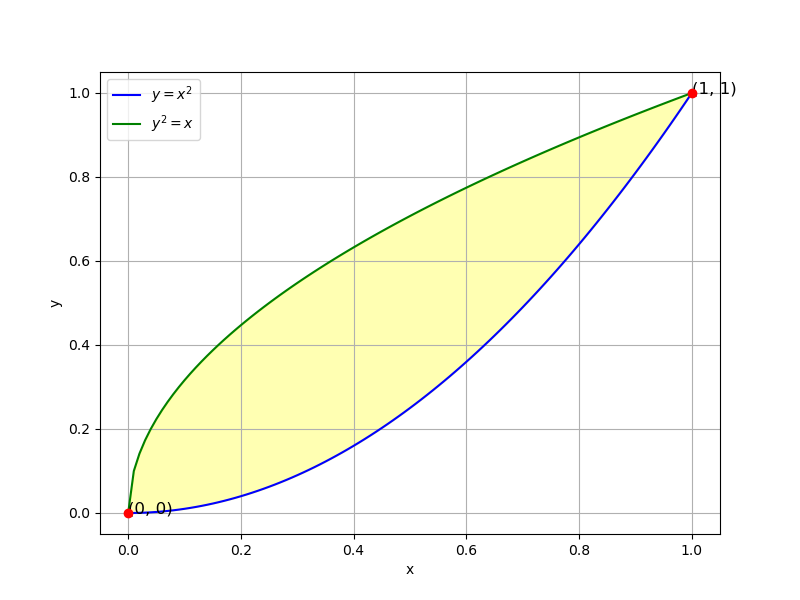
\includegraphics[width=1\columnwidth]{figs/Figure_1.png}
   \caption{Graph of the parabolas $y=x^2 \text{ and } y^2=x $ and the area enclosed between them}
   \label{stemplot}
\end{figure}
\end{document}
